\documentclass[11pt]{article}
\usepackage{fullpage}
\usepackage{graphicx}
\usepackage{float}
\usepackage{amsmath, amsfonts}
\usepackage[utf8]{inputenc}
\usepackage{parskip}
\usepackage{listings}
\lstset{
    language = Java
    }


\begin{document}
\begin{center}
{{\Large \sc Algorithms and Data Structures 02105+02326}}
\end{center}
\rule{\textwidth}{1pt}
\begin{description}
\item[Student name and id:] Roar Nind Steffensen (s144107)
\item[Teaching assistant:] Martin Hemmingsen
\item[Hand-in for week:] 4
\end{description}
\rule{\textwidth}{1pt}
 

\section*{Exercise M.1}

Insertion sort is implemented in java, and can be seen in the appendix.

\section*{Exercise M.2}

The generated program generates random sequences of length up to 250.000 integers.
The longest sequence (stored in an array) takes ~13 seconds to sort with the implemented insertion sort algorithm.

\section*{Exercise M.3 and M.4}

Plotting the length of the array vs the time to perform insertion sort we get figure \ref{fig:comparison}.

As expected the sorting time for insertion sort runs at $\Theta(n^2)$ (as seen when compared to the plot of $ax^2$), and is greatly outperformed by the default chosen sorting algorithm.

If we generate larger sequences of random integers, we can check the running time of the default sorting algorithm of java as seen in figure \ref{fig:default}. This shows that the running time for this sorting algorithm mainly follown $\Theta(n)$ although at large $n$ we it is uncertain to say if it is indeed $\Theta(n)$ or $\Theta(n \log n)$. This running time suggests that the algorithm uses either radix sort or an enhanced quicksort / mergesort. Inspecting the Arrays class, we see that the algorithm used is a double pivot quicksort. This algorithm should have a running time of $\Theta(n \log n)$, which might explain the higher times seen as n grows large.

\begin{figure}
    \centering
    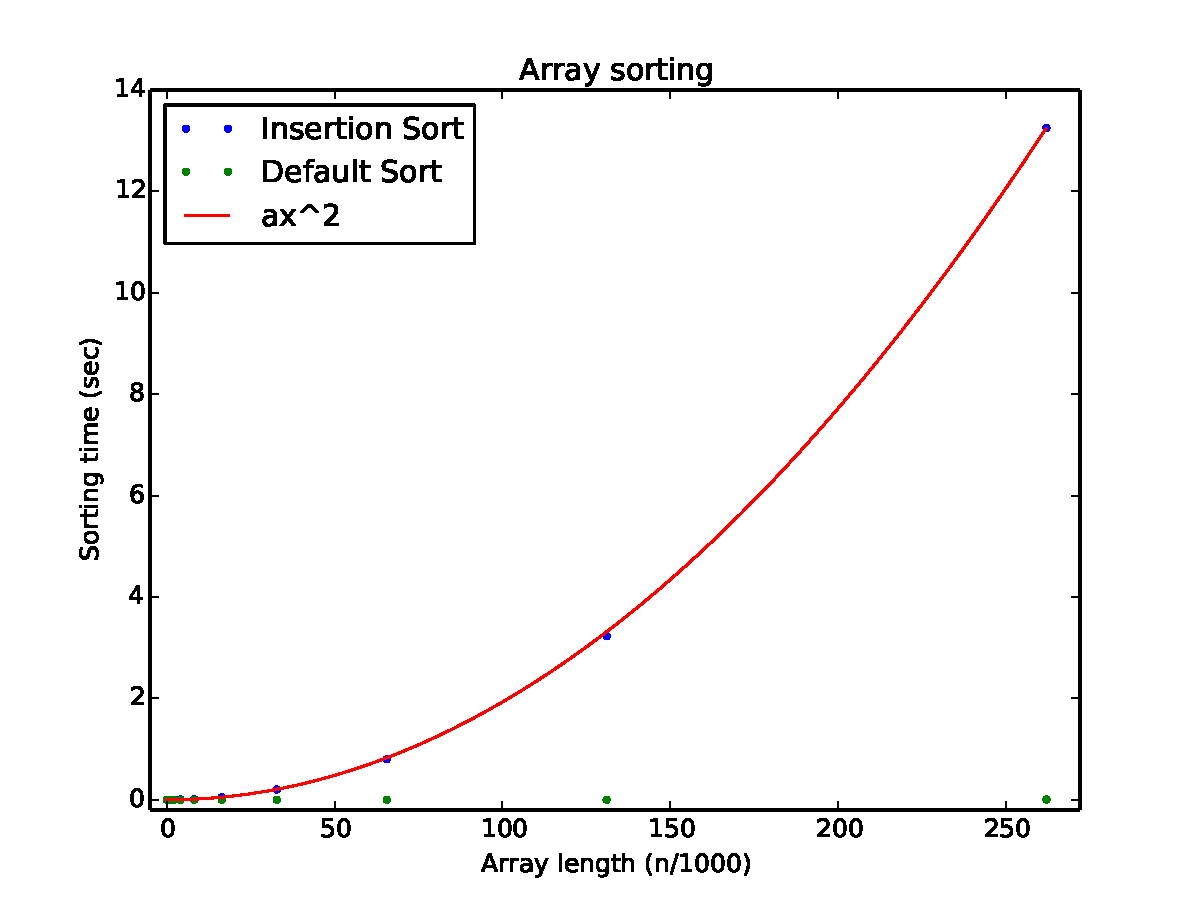
\includegraphics[width = 12cm]{SortingTime.pdf}
    \caption{Sorting times for insertion sort, and the default sorting algorithm in java.}
    \label{fig:comparison}
\end{figure}


\begin{figure}
    \centering
    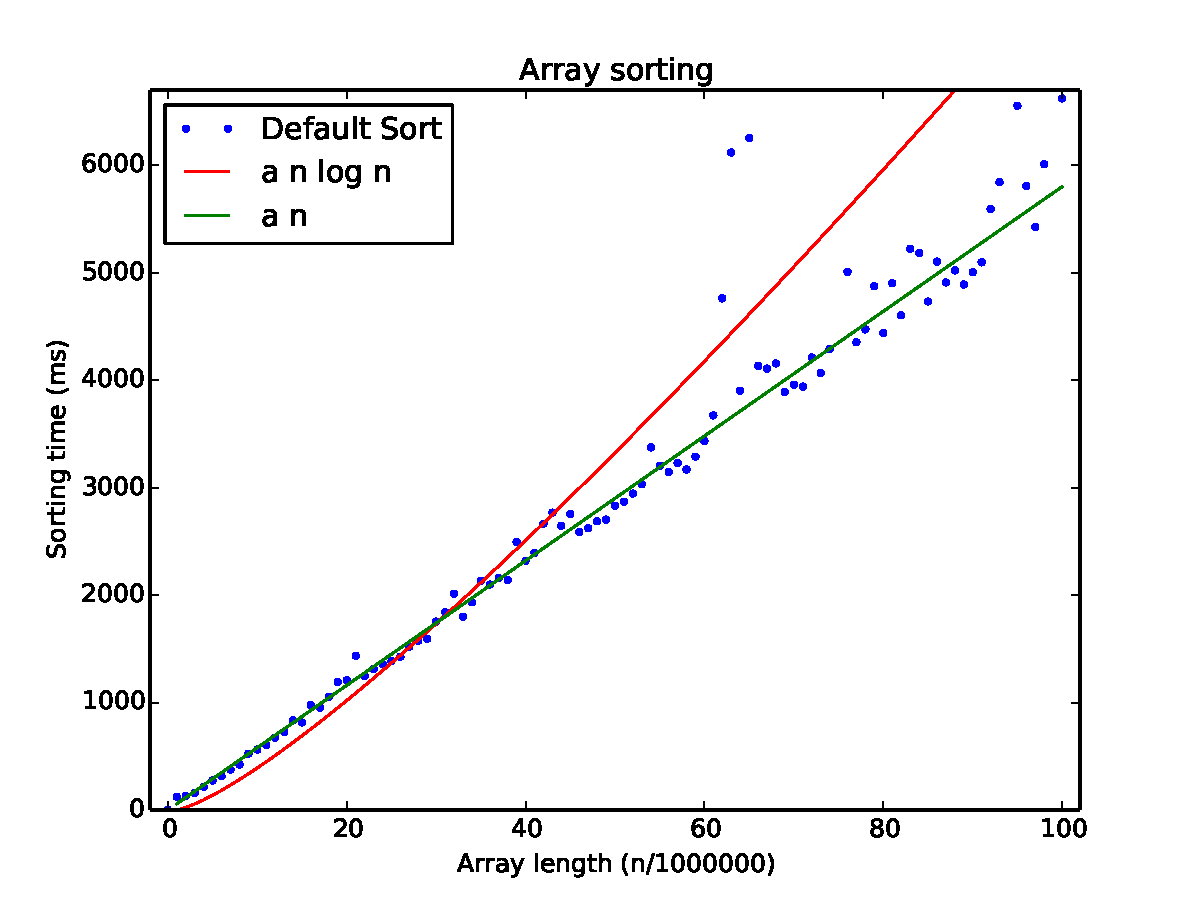
\includegraphics[width = 12cm]{Default}
    \caption{The default sorting algorhithm for java.}
    \label{fig:default}
\end{figure}


 \newpage
 
 \section*{Appendix}
 
 The implemented insertion sort is seen in the following java code:
 
 \begin{lstlisting}
public static int[] sort(int[] A) {
  if (A.length <= 1)
    return A;

  for (int i = 1; i < A.length; i++) {
    int j = i;
    while (j > 0 && A[j] < A[j - 1]) {
      int temp = A[j];
      A[j] = A[j - 1];
      A[j - 1] = temp;
      j--;
    }
  }

  return A;
}
\end{lstlisting}
 
\end{document}